\section{Photo-resistor}
\begin{figure}[H]
    \centering
    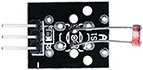
\includegraphics[angle=0, keepaspectratio=true, scale=1, width=200px, height=200px]{images/photosensor.jpg}
    %\caption{Caption}
\end{figure}
\subsection*{Description}
A photo-resistor is a light (brightness) dependant resistor. The photo-resistor is placed in series with a fixed value resistor, creating a voltage divider.

\subsection*{Pin mapping}
This pin mapping corresponds to the pins from left to right with the module pins facing towards you.
\begin{table}[H]
    \centering
    \begin{tabular}{|c|c|c|c|c|}
    \hline
    Index &Label &Type &Name &Description\\ \hline
    0 &S &Analog output &A0 &Photo-resistor output\\ \hline
    1 & &Source voltage &$V+$ &Module source voltage ($5V$)\\ \hline
    2 &- &Ground &GND &Ground\\ \hline
    \end{tabular}
    %\caption{Caption}
    %\label{tab:my_label}
\end{table}
\subsection*{Operation}
When light is shone on the sensor its resistance drops, conversely in low light conditions its resistance remains high (open circuit).

The output voltage at the analog pin (A0) will increase as the brightness or intensity of the light source increases until the photo-resistor acts like a short circuit. When there is no light hitting the sensor module the output at A0 will be zero.
\subsection*{Code}
Refer to listing \ref{python_photoresistor2}.
%\lstinputlisting[caption=test]{laser.py}